\documentclass{article}

% if you need to pass options to natbib, use, e.g.:
% \PassOptionsToPackage{numbers, compress}{natbib}
% before loading nips_2016
%
% to avoid loading the natbib package, add option nonatbib:
% \usepackage[nonatbib]{nips_2016}

\usepackage[final]{nips_2016}

% to compile a camera-ready version, add the [final] option, e.g.:
% \usepackage[final]{nips_2016}

\usepackage[utf8]{inputenc} % allow utf-8 input
\usepackage[T1]{fontenc}    % use 8-bit T1 fonts
\usepackage{hyperref}       % hyperlinks
\usepackage{url}            % simple URL typesetting
\usepackage{booktabs}       % professional-quality tables
\usepackage{amsfonts}       % blackboard math symbols
\usepackage{nicefrac}       % compact symbols for 1/2, etc.
\usepackage{microtype}      % microtypography
\usepackage{xcolor, graphicx, subcaption, float, enumitem, amsmath}

\newcommand{\selfnote}[1]{\footnote{\textcolor{red}{#1}}}
\newcommand{\domainDoubt}[1]{\footnote{\textcolor{teal}{#1}}}
\newcommand{\technicalDoubt}[1]{\footnote{\textcolor{blue}{#1}}}

\title{Commuter classification and behavior clustering: Beijing use case}

% The \author macro works with any number of authors. There are two
% commands used to separate the names and addresses of multiple
% authors: \And and \AND.
%
% Using \And between authors leaves it to LaTeX to determine where to
% break the lines. Using \AND forces a line break at that point. So,
% if LaTeX puts 3 of 4 authors names on the first line, and the last
% on the second line, try using \AND instead of \And before the third
% author name.

\author{
  Selene Baez  Santamaria \\
  \texttt{s.baezsantamaria@student.vu.nl}
}

\begin{document}
% \nipsfinalcopy is no longer used

\maketitle

\begin{abstract}
  Public transportation, centered on subway and bus networks, is an data-rich domain that can benefit from data mining and machine learning techniques. The classification of commuters versus non-commuters/occasional travelers can help government, transport management and operators to better target their policies in order to improve the transportation network in large cities. Furthermore, characterizing commuters by behavior clustering can bring deeper insight into their needs and routines as a whole. 
  This project proposes the usage of ensemble models for classification and clustering of public transport users. For this purpose, transit card data will be used, available from the city of Beijing, China. 
\end{abstract}

\newpage

\tableofcontents

\newpage
\section{Introduction}

\subsection{Urban public transportation}
% Why is public transportation important?
Urban public transportation includes systems that are available for use by anyone in urban areas. Its facilities are commonly composed by buses, subway/metro lines, light rails, tramways, trains, taxis and others. As a network, they provide service for the majority of citizens in urban areas.\citep{vuchic1900urban}

Figure \ref{fig:transportation/passenger} shows the passsenger transport usage, as million passengers per kilometer, in several different countries according to the Organisation for Economic Cooperation and Development (OECD). From all OECD countries, the United States, China, Germany, France, Italy, and the United Kingdom contitute the six countries with the most passenger transport, according to their reported data from 2015 or later.\cite{OECD2017passenger} 

\begin{figure}[H]
  	\centering
  	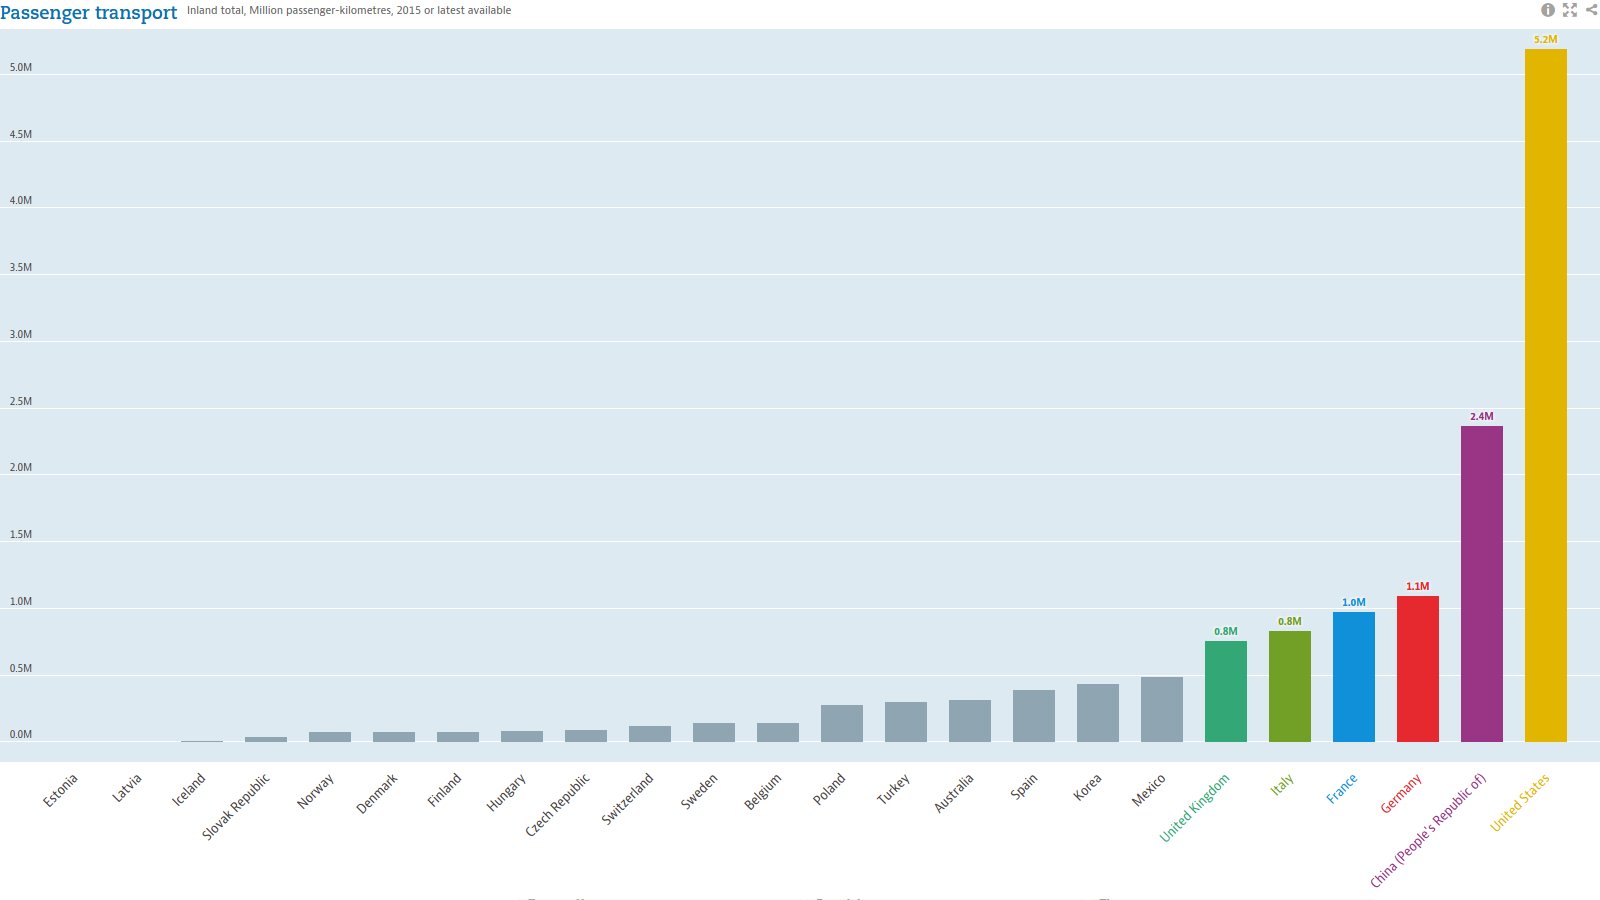
\includegraphics[width=\linewidth]{./images/OECD_passengers_absolute.png}
  	\caption{OECD countries and their passenger transportation data.}
  	\label{fig:transportation/passenger}
\end{figure}

Furthermore, historical data in Figure \ref{fig:transportation/passenger-trend} reveals the 15 years behavior for each of the aforementioned countries. Most of the countries show stability, with increase or decrease of less than 0.10 million passengers for European countries, and 0.5 million passengers for the United States. China, however, shows a trend with steep increase for most of the selected years. In fact, comparing to its less than 1.2 million passengers in 2000, China doubled its public transport usage to 2.4 million passengers in 2015. 
  
\begin{figure}
  	\centering
  	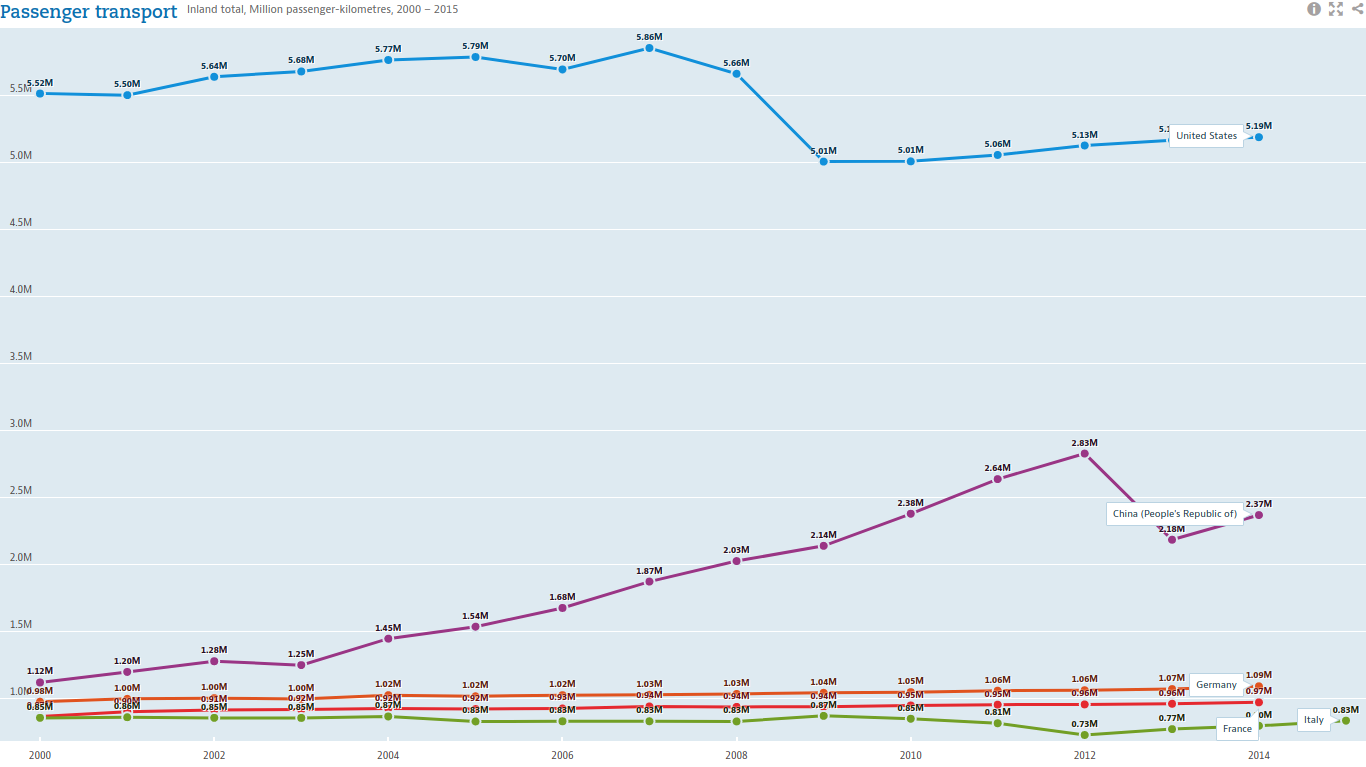
\includegraphics[width=\linewidth]{./images/OECD_passengers_increase.png}
  	\caption{Historical data for the top six countries with most passenger transport usage. China (top-left image) has the steepest increase overall.}
  	\label{fig:transportation/passenger-trend}
\end{figure}

Though it is a more sustainable alternative compared to private car usage, public transport usage has a significant environmental impact, affecting noise and air pollution. Diesel buses, which generally make up a major part of public buses, have large fuel consumption needs and contribute significantly to CO$_{2}$ emissions. Even eco-friendly alternatives such as hybrid diesel buses are sensitive to operating conditions, as their fuel consumption may increase by up tp 50\% when the on-board air conditioning is on.\cite{zhang2014real}

Consequently, public transportation directly relates to energetic demand, since its facilities are mostly petroleum or electrical based. In terms of global energy consumption, passenger transportation accounts for about 25\% of the total world energy consumption. Furthermore, the transportation sector consupmtion increases at an annual average rate of 1.4.\% \cite{eia2016energy} This may bring further economical implications for countries with high public transportation demand.

\subsubsection{Who are the commuters?}
% Self proclaimed commuters
A major proportion of public transport users is represented by commuters. These are regular users of public transit, with consistent spatiotemporal patterns in their travels. Driven by a routine, commuters travel back and forth from specific places, for example, from their home to work, school, or other similar locations. 

As commuters are frequent users of public transit, the  conditions of the public network directly influence their personal well being and generally impact their quality of life. Intuitively, if the commuting experience is unpleasant, daily travel can bring distress to commuters and/or even repel them from using the public transport at all. Several studies have looked into public transit evaluation from different perspectives, including commuters' needs \cite{mao2016commuting}. The most common aspects of it include: travel time, average speed, delays, accessibility, service coverage, crowded level, facilities quality, and fare rate. Weng et al \cite{weng2013bus} identified five indexes (Convenience, Rapid, Reliability and Comfort) that summarize commuters priorities when choosing to travel by public transport.
 
From both of the above, the large presence of commuters and their known needs and preferences, it follows that identifying commuters and addressing their needs can help in creating a sustainable public transportation network. Public transit stakeholders should be able to understand the commuters' demands and its dynamics, consequently bringing long term planning and policies for improving the overall commuting experience.

\subsection{The city of Beijing}
% Why is beijing a good (challenging, rich, valuable, relevant) use case?
The city of Beijing presents a special case of urbanization and rapid industrialization. This is reflected in a sudden population growth of 20\% per decade since 1960, with the largest increase of 44\% in the last ten years. The latest official census in 2010 reported the urban agglomeration of Beijing (including Beijing itself and its adjacent suburban areas) having a population of 19,612,368 people. The UN World Urbanization Prospects estimates the 2017 population at over 22 million inhabitants. \cite{world2016beijing}

As a result of the population explosion, many environmental and social resources are under pressure. From the environmental side, one of the most notable issues is related to air pollution, due to the significantly high pollutant emissions in the city \cite{zhang2016air}. Similarly, the city's downstream river pollution is serious, with most regions of the Yellow river being unable to comply with the lowest water quality standards. \cite{wang2015studies} 

On the aspect of social resources, one of the main complications is mobility. In Beijing, public transport is the dominant mode of transportation, accounted for 44.0\% of all trips compared to 32.6\% attributed to private cars \cite{mao2016commuting}. In 2008, the total ridership was 6.5 billion travels. Though the network is continually expanding, it is a fact that public transport is overcrowded, constantly reaching over 100\% capacity \cite{beijing2009research}.

Beijing public transport is composed of buses, subway and bicycles. The three types can be accessed by using a single smart card. 

\begin{description}
\item[Bus:] In 2015, there were 876 bus lines with 23,287 buses in operation. The bus network is the most extensive mode of transportation, expanding over 20,186 km. It observes an average daily traffic volume of 10.98 million passengers, with the highest daily volume reaching 13.07 million on one day. \cite{beijing2016annual}

\item[Subway:] The Beijing subway has 18 lines with 334 stations, of which 53 are transfer stations. In 2015 it had an operating length of 554 km, with 5,024 vehicles running. \cite{beijing2016annual} Its network is split by two operators: the state-owned Beijing Mass Transit Railway Operation Corp (operating 15 lines), and the joint Hong Kong venture Beijing MTR Corp (operating 3 lines).

Beijing's subway has an average daily traffic volume of 9.11 million passengers, with a maximum recorded volume of 11.66 million passengers. As such, it is the second busiest metro system in the world, providing 3,410 million annual journeys. Compared to the service provided in 2012, the system observed a 39\% increase in usage by 2014. It is also the second longest metro network, surpassed by Shanghai by only 21 km.  \cite{uitp2015world} 

\item[Bicycles:] Beijing first implemented public bicycle systems in 2012. As of 2015, in total, 67,000 bikes are available for rental with 2,700 pick up/drop off points spread across the city. \cite{beijing2016annual}
\end{description}


\subsection{Smart cards and Big Data}
Smart cards present us with a straightforward way of massively collecting daily data. In the last years, smart card systems have become more popular in the Transportation domain, making it possible to monitor travelers transactions and facilitating fare collection. Several cities have implemented such systems, for example the Octopus card in Hong Kong\cite{chau2003octopus}, Oyster card in London \cite{blythe2004improving}, OV-chipkaart in The Netherlands \cite{de2008analysis}, and Yikatong card in Beijing \cite{chan2010tactical}, to name a few.

In Beijing, over 90\% of public transit users are smart card holders. There is a significant incentive for using the Yikatong smart card since bus rides are heavily subsidized (users have only to pay 50\% of the full price)\cite{ma2017understanding}. Moreover, the Yikatong smart card system is also integrated with taxi, electricity and sewage payments, making it convenient to use as a general paying method.

\paragraph{Data quantity}

Placed in context, public transit systems serve at least hundreds of users daily, where a typical user performs several trips a day, every day. On the specific case of Beijing, there are hundreds of thousands of smart cards gathering between 5 and 16 million records (trips) a day, among a large complex network containing thousands of routes and tens of thousands of stops. 

\paragraph{Data quality}

However, though smart cards exponentially increase the quantity of data, they do not completely guarantee its quality. As is, some aspects of the trips cannot always be faithfully recorded but are inferred (for example, the transfers between the subway system when no check-in/out is done at changing trains). Furthermore, some fields are sometimes simply missing or incorrectly recorded due to malfunctions and situations out of control. 


Given the large amounts of data collected and its nature, the analysis of such becomes challenging. Transit smart cards are capable of recording spatiotemporal information at an individual level over long periods of time. This generates a large volume of historical data that only tailored big data techniques can deal with. 

\subsection{Project motivation}
This project performs an interdisciplinary study between the areas of Artificial Intelligence and Metropolitan Transportation. It is focused on introducing data mining techniques to a data rich domain. 

% Each science benefits
The area of Artificial Intelligence is able to provide dozens of prediction algorithms. Though constantly under refinement, it is time for state-of-the-art techniques to be applied, tested and validated under real and large impact situations to test their ability to deal with noisy streams. Comparably, given the ever growing complexity of urban mobility, domain experts must focus on analyzing trends and insights instead of curating and making sense out of raw data. As such, introducing these state-of-the-art techniques into the Metropolitan Transportation domain can aid to unravel massive human behaviors and reveal patterns and trends in mobility.

\subsubsection{Societal context}
% description, prediction and preescription
Identifying and analyzing mobility patterns may have different goals, from description, prediction or prescription, all of which affect their stakeholders directly. 

A descriptive analysis determines how do people use the public transit. It can pinpoint chaotic hotspots in the city, peak hours, popular routes or other behaviors. A predictive analysis investigates how will people use the transit in the future or under new circumstances. For example, public transport usage projections in the years to come directly affects environmental models trying to improve air and water quality, energetic demand or other natural  and economic resources.

Finally, a prescriptive analysis focuses on how should the different stakeholders deal with mobility behaviors. For example, the government as well as transport management and operators would gain invaluable spatial and temporal insights regarding commuters' behaviors. This insight may lead to tangible results, including policies for increasing the efficiency of the public transit network, adjustable travel fares tailored to the most relevant mobility patterns, incentives to relieve peak hours and thus traffic congestion, urban planning for residential and industrial land use, and others.

Given that Beijing has a widely spread data collection system, combined with formidable institutions capable of introducing new measures in their public transportation network, this city is an excellent use case where the results of an in-depth study can generate actionable plans and bring benefits in the short and long term.

Furthermore, the social context of Beijing presents specific opportunities for improvements where the full power of data analysis and its impact can be tested. 

For example, the city of Beijing faces a large imbalance between residential and working areas. Due to urban expansion, most residents have been forced to move to suburban areas due to the lack of affordable housing, regardless of having their work environments within the six Ring Roads \cite{zhou2014commuting}. Investigating and targeting this group could alleviate the pitfalls of long distance commuting. 


\subsubsection{Scientific context}
% Improve individual and collective analysis
Mobility patterns in metropolitan areas follow complex swarm behaviors. Based on individual travels and routines, travelers exhibit distinguishable characteristics on a larger scale. Both individual and collective levels of understanding are crucial for Transportation experts. In order to explore both levels, Metropolitan Transportation studies typically focus of the usage of surveys. These surveys are targeted to reach travelers on an individual level, while large scale indicators and aggregated data are taken to investigate their collective behavior. 

These methods have several disadvantages. On the one hand, surveys are costly to implement, and in general have problems related to small non-representative samples. Even when these problems are escaped, the usual quality versus quantity trade off is present, reducing the confidence of the collected information. On the other hand, large scale measurements (i.e. total passenger flow) miss the interactions between individuals that cause the collective behavior.

On top of this, an important consideration on the Metropolitan Transportation domain is that the data collected by smart cards is unlabeled. This means that traveling behaviors are not assigned to known specific categories, making it hard to validate and evaluate. Typically, this issue is address by asking some sample users -via surveys- how they categorize themselves (for example, if they consider themselves to be commuters) and then extrapolating this profile to new users. However, self-reported data by itself has bias problems, therefore introducing noise or false patterns. 

Fortunately, the field of pattern recognition has seen major development in the last years. Nowadays, there exist machine learning and other data mining methods specialized in analyzing disaggregated complex information. Data analysis can be as general is specialized as needed, producing reliable and comprehensible information and visualizations. Furthermore, unsupervised tools have arisen that find patterns based on the data alone, thus being independent from the aforementioned biases.


\subsection{Thesis organization}
The rest of this thesis is organized as follows: On the next section we perform a \textit{Literature review} to explore previous work on mining smart card transit data. We also summarize current representation and pattern recognition methodologies for dealing with complex spatiotemporal data.  

Subsequently, we establish the \textit{Research framework} where we explicitly state the objectives and research questions of this project. As a result, we limit the project's scope and clearly define the most important terms to be used. 

We continue to describe the \textit{Methodology} thoroughly. This consists of an extensive description of the data and its characteristics, our proposed 3 dimensional representation for spatiotemporal data, and the data mining approach to follow, including supervised and unsupervised learning techniques for dimensionality reduction and pattern recognition.

Following this, we identify three distinct stages of the project: \textit{Data preparation and preprocessing}, \textit{Commuters identification}, and \textit{Traveling behavior clustering}. In the \textit{Data preparation and preprocessing} section we describe the pipeline for processing raw data, extracting trip attributes and finally creating the proposed 3D representation of an user's traveling behavior. 

The section on \textit{Commuters identification} describes a supervised learning approach to classifying labeled data, using feature selection and ensemble models. Its counterpart, the section on \textit{Traveling behavior clustering} describes an unsupervised  learning approach to recognize similar traveling behaviors, using feature extraction (by means of an autoencoder) and clustering algorithms. 

Finally, we gather conclusions regarding the proposed representation. We compare both supervised and unsupervised approaches and explore future work opportunities. 

\newpage
\section{Literature review}
In this section we look at studies within the last decade that are related to smart card transit data. First, we summarize the approach and the most relevant findings of each paper in order grasp a broad view of the Transportation domain. Secondly, we explore representations for spatiotemporal data and compare the way traveling behavior is usually represented in the Transportation domain, and other types of representations available in the Artificial Intelligence domain. Thirdly, we discuss techniques for pattern recognition through supervised and unsupervised learning. Finally we explore some pioneer work in end-to-end learning. 

\subsection{Data mining on transit card data}
% What questions and approaches are common. How do they interpret traveling behavior? What's the volume of data?
With the introduction of smart card systems in large cities, several studies have aimed to extract knowledge from the large amounts of data collected. Many of this studies focus on analyzing traveling behavior, which is regarded as a spatiotemporal mobility pattern. Though different in their methodology, results concerning commuters are duplicated across studies. As the spatial and temporal regularity of commuters' travel behavior is evident in their smart card data, they pose an excellent opportunity of study.

Morency et al. study spatio-temporal variability in Canadian smart card data. On the one hand, they examine spatial variability by measuring the number of distinct stops a smart card user visits, and the frequency of each stop. On the other hand, they examine temporal variability by clustering the boarding times of each type of smart card. Using these features, they observe the week to week variability for each of the five types of transit card available (Adult-interzone, Adult-express, Adult-regular, Elderly and Student). Their findings show that commuter types of cards visit a smaller range of bus stops compared to non-commuter types. Therefore, a small number of stops account for a high proportion of commuter's boardings. Additionally, commuters have the highest proportion of zero-boarding days on weekends \cite{morency2007measuring}.

%Density Based Scanning Algorithm with Noise to classify travelers according to their travel patterns.  \cite{ma2013mining}

Bhaskar et al. are concerned with passenger segmentation using Australian smart card data. First, they perform a two level DBSCAN algorithm for investigating spatial patterns, where the first level clusters Destination stops and the second level clusters Origin stops.  From this they extract frequent Origin-Destination (O-D) pairs. Separately, they applied DBSCAN to temporal features to determine most frequent boarding times.  As such, they characterize each user by the percentage of journeys they perform between the regular O-D, and the percentage of journeys they perform during their habitual times. Users with at least 50\% spatial and temporal regularity are thus classified as transit commuters; while users with no evident spatial or temporal pattern are classified as irregular passengers. The authors find that while most (64\%) of the passengers riding the public transit are irregular passengers, it is transit commuters who bring the most (46\%) revenue. Furthermore, they find that irregular passengers prefer high frequency routes significantly more than transit commuters, arguing that commuters are usually on a time habit, and thus are more willing to check and adapt to public transit timetables. \cite{bhaskar2015passenger}

Tu et al. follow a supervised learning approach to classify public transit users in Beijing as commuters or non-commuters. In order to produce labeled data, they convey an online survey asking for travel patterns and smart card ID. Matching the ID to the journeys recorded by smart card during the span of one week, they collect records associated to 978 travelers. The classification is then performed by a Support Vector Machine (SVM), which reaches up to 94.24\% accuracy. \cite{tu2016impact}

Langlois et al. present an innovative representation for smart card data. Using four weeks worth of data from London Oyster cards, they represent the card information as a time-ordered sequence of inferred activities.  11 clusters are found and characterized by evaluating socio-demographic variables like age, employment, annual household income, children per household and vehicles per household. The authors further grouped the clusters under "working day", "home bound", "complex activity pattern" and "interrupted pattern" categories. Their findings show that four clusters, grouped under the "working day" category have significantly different activities during weekdays as compared to weekends, with some avoiding transit during the weekends and others visiting different areas.  Four more clusters, grouped under the "home bound" category, are characterized by staying mostly at their primary area and low number of traveled days. \cite{langlois2016inferring}

One of the latest work on the field corresponds to Ma et Al. The objective of their work is to determine a scoring function for travelers that can correctly identify them as commuters, or non-commuters. In their work, they cluster stops using an improved DBSCAN algorithm. They engineer features for representing the frequency in which travelers follow spatio-temporal patterns. Travelers are then clustered according to these features following the ISODATA algorithm. As an output of the clustering, optimal cutoff levels in the scoring function were determined. As a result, evaluating a traveler does not depend on clustering centroids, but only on calculating the commuting score. This, as expressed by the authors, reduces computing time and treats each traveler independently from the others, which is not true for clustering algorithms \cite{ma2017understanding}.

A common practice, as used by \cite{ma2017understanding}, \cite{langlois2016inferring}, and \cite{morency2007measuring} is to divide the day into -hourly or half-and-hour- time bins. Bhaskar et al. recognize this as a problem in the field, by pointing out that this design choice segregates journeys from 9:59 AM and 10:01 AM even though they intuitively belong to the same behavior. 

\subsubsection{Volume of data}
The volume of data collected by smart card systems is massive and is usually impossible to analyze all of it at once. The volume of the samples analyzed by previous work ranges from hundreds of smart cards to tens of millions of smart cards, leading to up to hundreds of millions of individual smart card transactions. The details are summarized in Table \ref{table:volumeData}.
 
\begin{table}[H]
\centering
\begin{tabular}{||c c c c c||} 
 \hline
 Authors & Year of publication & Records & Unique smart cards & Time span \\ [0.5ex] 
 \hline\hline
 Tu et al. \cite{tu2016impact} & 2016 & 8,067 & 978 & one week \\ 
 Morency et al. \cite{morency2007measuring} & 2007 & 2.2 million & 7,118 & 277 days \\
 Langlois et al. \cite{langlois2016inferring} & 2016 & 3 million & 33,026 & four weeks \\
 Bhaskar et al. \cite{bhaskar2015passenger} & 2015 & 34.8 million & 1 million & 4 months \\ %, working days only
 Ma et al. \cite{ma2013mining} & 2013 & Unknown & 3 million & one week \\
 Ortega \cite{ortega2013classification} & 2013 & 65 million & 5.7 million & one week \\
 Ma et al. \cite{ma2017understanding} & 2017 & 364 million & 18 million & one month\\ [1ex] 
 \hline
\end{tabular}
\caption{Volume of data analyzed by different authors}
\label{table:volumeData}
\end{table}

Trade off between several cards and short period or few cards over long period. \selfnote{expand}

\subsection{Representing spatiotemporal data}

\subsubsection{Traditional feature engineering}
Human mobility is intrinsically tied to spatio-temporal properties. Still, the greatest amount of studies analyze public transit journeys by separating spatial features from temporal features. In general, scalar aggregated features are used for users characterization. Some examples are:

\begin{itemize}
\item \textbf{Frequency indicators:} number of traveled days \cite{bhaskar2015passenger} \cite{langlois2016inferring} \cite{ma2017understanding}, number of journeys \cite{bhaskar2015passenger}, number of times a stop was visited \cite{morency2007measuring}, number of days with zero boardings \cite{morency2007measuring}, most frequent home/work stop \cite{ma2017understanding}, most frequent home/work route \cite{ma2017understanding}, most frequent departure time from home/work \cite{ma2017understanding}, number of trips to the most frequent home/work stop\cite{ma2017understanding}, number of trips following the most frequent home/work route \cite{ma2017understanding}, number of trips during most frequent departure time from home/work \cite{ma2017understanding}

\item \textbf{Range/coverage indicators:} distinct stops visited \cite{morency2007measuring}, spread of days between the first and last journey \cite{langlois2016inferring}

\item \textbf{Calendar-based indicators:} observed day \cite{morency2007measuring}, day of week \cite{morency2007measuring}

\end{itemize}


\selfnote{disadvantages of hand engineered aggregated}


\subsubsection{Feature extraction}
Automatically extracting features. Dimensionality reduction. 

\textbf{Principal Component Analysis}

Different from all of the above, Langlois et al. follow a unique methodology for engineering features. First, they represent the travel data per user using a three dimensional matrix where $x$ represents the day in the four week period, $y$ represents the hourly time bin, and $z$ represents the area where the inferred activity took place, encoded as a one hot vector. The authors perform Principal Component Analysis (PCA) for dimensionality reduction, based on Eagle and Pentland's eigenbehaviours \cite{eagle2009eigenbehaviors}. An analysis of the average correlation of the first 13 components, results in the selection of the first 8 components as the most informative and stable. The projections of a user sequence onto these components (called weights) constitute the features to be clustered using k-means. \cite{langlois2016inferring}

\textbf{Autoencoders}

Autoencoders map high dimensional data to low dimensional spaces 


\subsection{Pattern recognition on spatiotemporal data}
% Supervised and unsupervised learning

\subsubsection{Classifying algorithms}
The domain of Metropolitan transportation faces a specific problem: although smart card systems have allowed massive collection of data, this data is not labeled regarding commuting behaviors. Additionally, obtaining labels for smart card data is expensive and unreliable, since it has to be acquired through surveys or interviews. Furthermore, even when labels are obtained, the amount of labels obtained is often insufficient for big data analysis. It is due to these reasons, that most studies are inclined to used unsupervised learning techniques. 

One of the few studies that uses labeled data corresponds to Tu et al. They obtain 978 labeled records, with an almost equal distribution of records over both classes (49.18\% related to commuter samples and 51.82\% related to non-commuter samples). They solve the issue of limited samples by selecting a model that is not heavily affected by sample size: Support Vector Machines. Their results report a 94.24\% accuracy over a test set of 295 samples. 

\subsubsection{Clustering algorithms} 
If labeled data is not available, then unsupervised learning techniques must be applied. There is a large variety of clustering algorithms available nowadays, however not all of them are suitable for all types of data and purposes.

\textbf{Hierarchical clustering}

Langlois et al. use agglomerative hierarchical clustering for areas clustering. In order to infer the user-specific activities, all stops or stations visited by each user are clustered by merging the two closest areas until a threshold distance is reached. Their algorithm also considers the distance between stops and the frequency of travel between them. Therefore, different activities are likely to be associated with different areas \cite{langlois2016inferring}.

\textbf{Partitional clustering}

K-means algorithm is the most widely used method for partitional clustering. It requires having a predefined number of clusters to fit the data to. 

Morency et al. use K-means for clustering hourly boarding times according to card type. They apply Hamming distance (representing the percentage of data between two elements) and a combination of batch and online updates. Through empirical tuning, they select to find four clusters per card type. It is worth noting that by using a card-day unit, they allow a card to belong to a different cluster according to the day of travel. As every card type is composed of four boarding patterns, travelers are not restricted to follow a routine everyday, but can exhibit different behaviors on different days. For example, the Adult-regular card type contains a 9:00AM-and-5:00PM-boarding cluster and a no-boarding cluster. Thus, a user of this card could belong to the first cluster on weekdays and to the second cluster on weekends.  \cite{morency2007measuring}

Bhaskar et al. apply K-means for binary classification purposes. As such, they classify frequent and infrequent transit users, using the number of traveled days and the number of journeys made as features. Unfortunately, K-means performs poorly since no distinct clusters are evident. The most likely cause for the previous is the strong correlation between traveled days and journeys, combined with the authors oversight of whitening and standardization techniques. \cite{bhaskar2015passenger}

Langlois et al. use K-means to find clusters of activity sequences. They employ specialized sampling techniques, like bootstrapping, to deal with big data.  Moreover, they tune the algorithm parameters using the DB-index, which is the ratio of the within cluster distances to the across cluster distances. They find two optimal number of clusters (4 and 11), out of which they select the largest to provide the most detailed segmentation. They further perfection the algorithm by using k-means++initialization over 150 replications. Additionally, this paper acknowledges that clustering techniques are sampled based, which means different samples may find different optimal solutions. The authors validate their approach by analyzing the stability of the clusters over samples obtained at different points in time. By extracting the same number of clusters and fitting the samples to each set, they find that 91\% of users are assigned to their equivalent clusters. \cite{langlois2016inferring}

\textbf{Density based clustering}

Density based algorithms excel at dealing with anomalies, since they ignore low density areas and interpret them as noise. They do not required a redefined number of clusters and adapt to find clusters of any size. The required parameters for DBSCAN are a maximum reach distance $\epsilon$ and the minimum number of points per cluster.

Bhaskar et al. use three DBSCAN algorithms to cluster Origin stops, Destination stops, and boarding times. For each of the previous, they tune the algorithm parameters by fixing a domain reasonable $\epsilon$ (1000 m walking distance or 5 min variance in boarding time), and selecting the minimum points by comparing the percentage of data considered to belong to any cluster as opposed to data considered to be noise given the par-specific parameters \cite{bhaskar2015passenger}. 

Ma et al. use an improved DBSCAN algorithm to cluster bus/subway stops. In their approach, abnormal stops are not considered noise, but are allowed to be re-clustered by splitting large clusters into several smaller clusters. 

Though clustering algorithms are common in the field, they are not always used for classifying users. For example, Bhaskar et al. use density based clustering for engineering regularity features. However, the classification of users is rule-based according to which feature (spatial or temporal regularity) is stronger in each user \cite{bhaskar2015passenger}. Morency et al. use partitioning clustering to characterize existing user categories according to their boarding times \cite{morency2007measuring}. 

As a conclusion, we note that while there has been research applying basic clustering and classification algorithms, most studies lack further specialized data mining techniques for preprocessing data, tuning algorithms parameters, and/or visualizing results. 


\subsection{End to end learning}
Learned representations, and learned underlying structure (patterns)

DEC with end to end learning. Propagate error from clustering


\newpage
\section{Research framework}
The underlying goal of this project is to find an accurate spatiotemporal representation for traveling behavior while accounting for big data constraints and the inherent data nature. The main two objectives are:

\begin{description}
\item[Objective 1] To identify commuters based on their routines. \label{eqn:obj1}
\item[Objective 2] To identify popular travel behavior patterns. \label{eqn:obj2}
\end{description}

Combined, these objectives identify and characterize commuters in the city of Beijing by using one month worth of smart card data. 

\subsection{Research questions}
The main objective is further broken down into answering the following research questions: 

\begin{enumerate}

\item How can spatiotemporal features be analyzed as a unit?

\item What are the most relevant features when identifying commuters?

\item How accurately can commuters and non-commuters be identified using an ensemble model? 

\item How many distinct behaviors are present among public transport users in Beijing?

\item How does feature selection and feature extraction compare to each other in the transportation domain?

\end{enumerate}

\subsubsection{Definition of terms}
A commuter is a public transit user whose smart card data reveals repeatable patterns in time and space. Though commuters are usually associated with Monday to Friday 9:00am to 5:00pm schedules, in this work we extend the definition to any routine travel pattern. This flexibility allows us to include travelers with stable yet rare commuting schedules, such as night workers, weekend workers and evening workers.

A trip is a sequence of smart card transactions, including transfers, performed by the same user to travel from an origin to a destination. A trip is also represented as a record in the data, as it will be further explained in Section \ref{sec:data}

A transfer is a change in transportation mode, or a change in vehicles whenever a smart card has to be checked within the same transportation mode. Transportation modes include Bus, Subway, and Bike. 

We make the assumption that smart card IDs and users have a one to one relationship, meaning each user has exactly one card and each card is used by exactly one user. As discussed with domain expert Quian Tu, although some people may own more than one card, this is a minority. Thus, the assumption holds for the majority of travelers. 

\subsection{Scope and structure}
This project is divided three main stages: 

\begin{description}[align=left,labelwidth=2cm]
\item[PART I: Prepare and preprocess the data using Big Data techniques] In this part we focus on research question 1. Techniques for cleaning, knowledge extraction, categorization, patching and standardization are used and tailored to the data. From this, we build an appropriate 3 dimensional representation for each user's traveling behavior. This part corresponds to Section \ref{sec:partI}.


\item[PART II: Classify commuters versus non-commuters by using an ensemble model]  In this part we focus on research questions 2 and 3. First, we perform feature selection in order to identify the most informative features and disregard redundant information. An extensive analysis of spatiotemporal properties is be done, combining transportation domain knowledge and statistical tools. Later, we create a classifier using ensemble models and discuss its performance. This part corresponds to Section \ref{sec:partII}


\item[PART III: Users clustering according to patterns in their travel behaviors.]  In this part we focus on research question 4. First, we do feature extraction with the goal of reducing the dimensionality of the data. This is done via a convolutional autoencoder. Finally, we cluster the low dimensional representation using k-means clustering and do cluster analysis to understand the underlying pattern of each cluster. This part corresponds to Section \ref{sec:partIII}
\end{description}

Figure \ref{fig:flowchart} displays a flowchart for the stages and their connection.

\begin{figure}[H]
  \centering
  \includegraphics[width=\linewidth]{./images/flowchart.png}
  \caption{Project flow}
  \label{fig:flowchart}
\end{figure}

\newpage
\section{Methodology}
\subsection{The data}
\label{sec:data}
Every record in the data represents a trip performed by a specific smart card. As such, it contains the following data fields:

\begin{itemize}
\item Data date: Year, month and day that the trip was made
\item Card code: Card identification number
\item Path link: Mode of transportation. B stands for bus, R for subway, Y for bicycle. Transfers between modes are shown by a dash. \footnote{Example: B-B represents a Bus to Bus transfer.} 
\item Travel time: Time spent in vehicles, measured in milliseconds
\item Travel distance: Distance traveled, measured in meters as performed by route. 
\item Transfer number: Number of changes in travel mode during the trip. 
\item Transfer total time: Total time spent in transfer, measured in milliseconds\item Transfer average time: Time spent in transfer, divided by number of transfers. Measured in milliseconds
\item Start/End time: Time stamp of when the trip started/ended. Date and time up to milliseconds precision
%Traffic zones
\item On/Off small traffic area: Integer ranging from 1 to 1911
\item On/Off middle traffic area: Integer ranging from 1 to 389
\item On/Off big traffic area: Integer ranging from 1 to 60
%Municipal zones
\item On/Off ring road: Integer ranging from 1 to 6
\item On/Off area: Integer ranging from 1 to 18
\item ID: record identification number created by joining the following: hour of the beginning of the trip | time stamp of beginning of the trip | card code performing the trip
\item Transfer detail: Mode of transportation, as well as line/route number and stations for boarding and alighting. More detail provided in Section \ref{sec:tripParsing}
\end{itemize}

Full privacy of card users is ensured, as there is no personal data linking card codes to specific individuals. 

The traffic zones (small, middle and big areas) are divided by the Beijing Municipal Institute of City Planning and Design (BICP). They are specific in different degrees, as shown in Figure \ref{fig:data/traffic_zones}. In general, the division principles correspond to the geopolitical environment and administrative planning, for example roads, villages and others. The 6 ring road and 18 areas districts are divided by the Beijing Municipal Government. The division is unique in Beijing. The 18 districts and counties are shown in Figure \ref{fig:data/18areas}. According to domain expert PhD. Liang Quan, these divisions are sufficiently informative for traffic analysis \cite{liang}.

\begin{figure}[H]
  \centering
  \begin{subfigure}[b]{.3\textwidth}
  	\centering
  	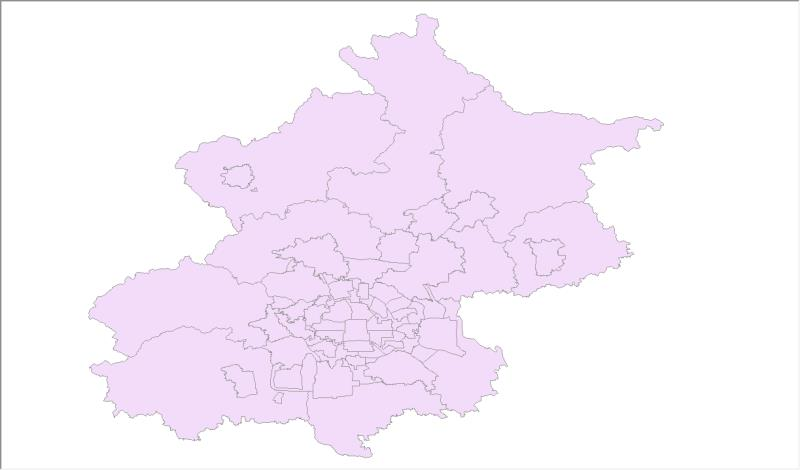
\includegraphics[width=\linewidth]{./images/big_traffic_zone.jpg}
  	\caption{Big zones}
  \end{subfigure}
  \begin{subfigure}[b]{.3\textwidth}
  	\centering
  	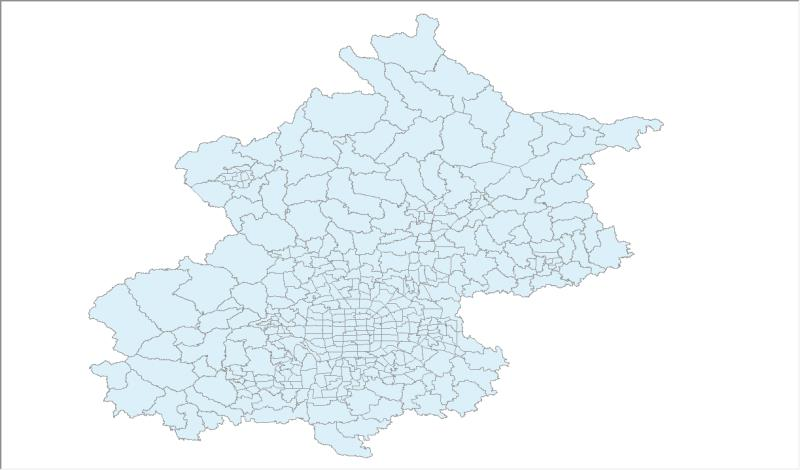
\includegraphics[width=\linewidth]{./images/middle_traffic_zone.jpg}
  	\caption{Middle zones}
  \end{subfigure}
  \begin{subfigure}[b]{.3\textwidth}
  	\centering
  	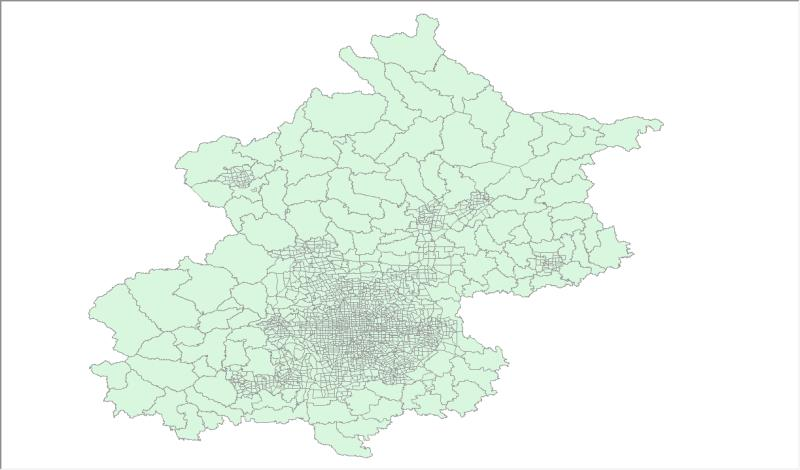
\includegraphics[width=\linewidth]{./images/small_traffic_zone.jpg}
  	\caption{Small zones}
  \end{subfigure}
  \caption{Traffic zone division}
  	\label{fig:data/traffic_zones}
\end{figure}

\begin{figure}
  \centering
  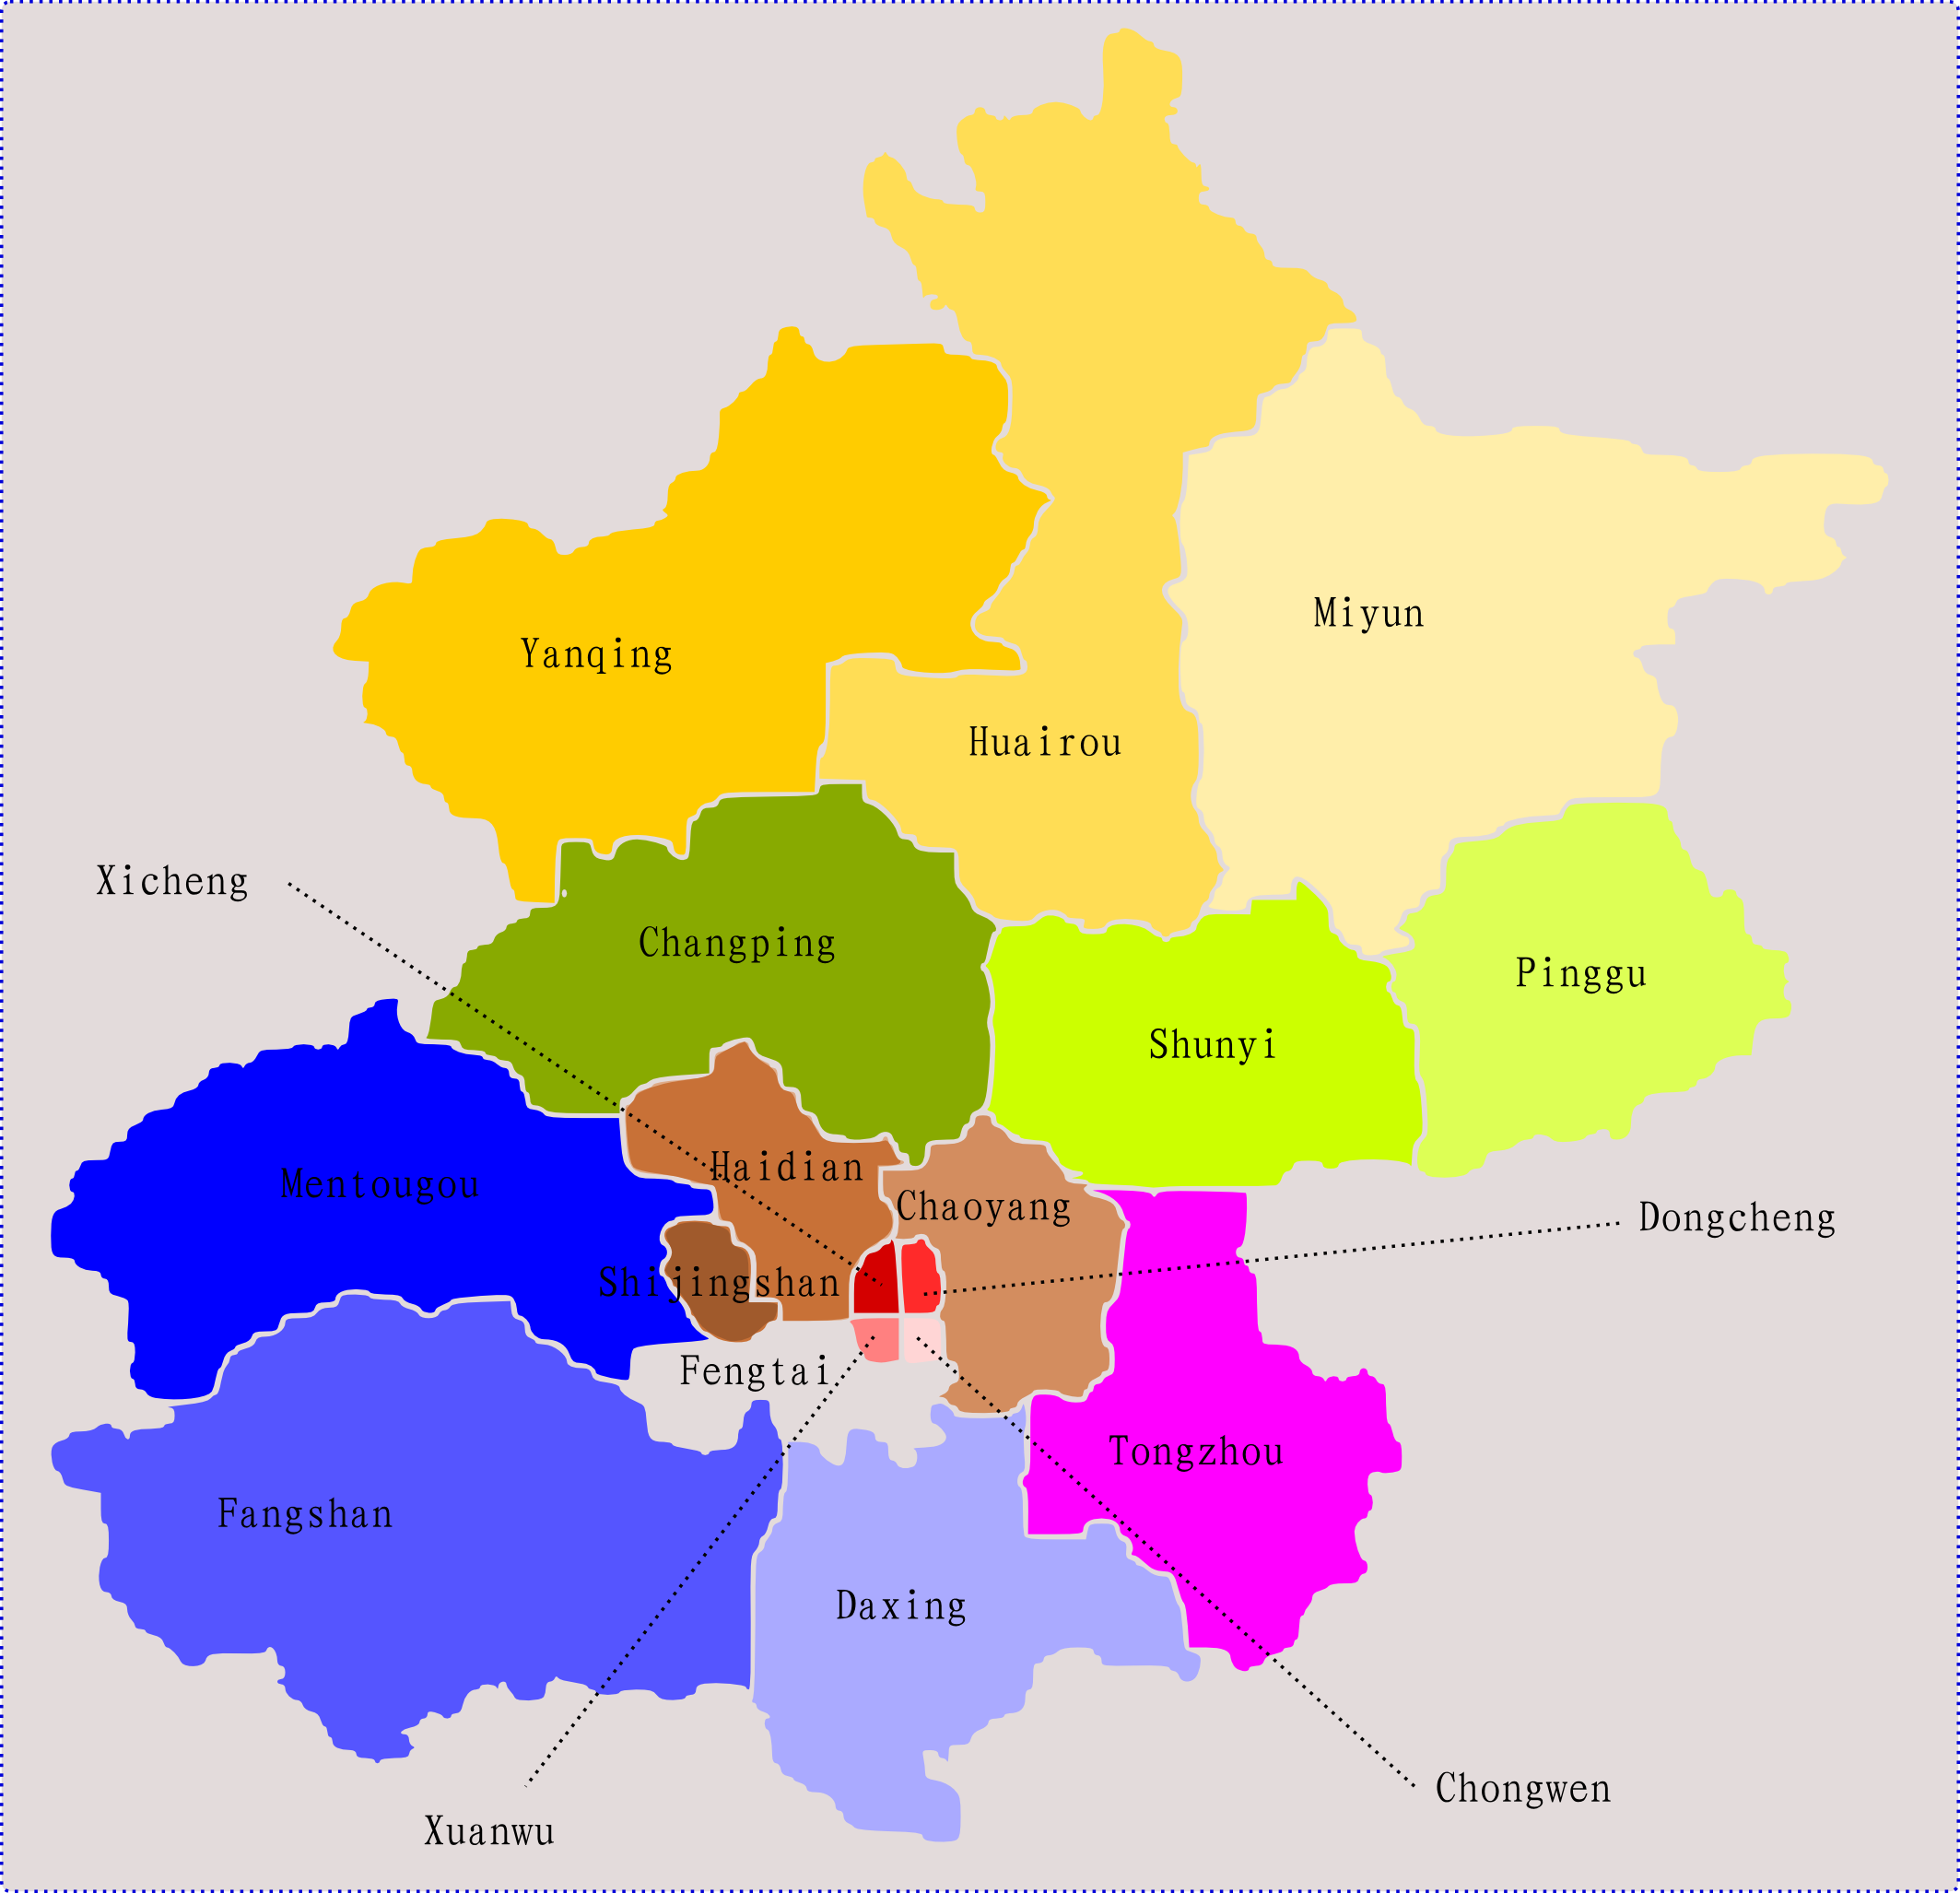
\includegraphics[width=.8\linewidth]{./images/beijing_18areas.png}
  \caption{Beijing's Districts and its Counties}
  \label{fig:data/18areas}
\end{figure}

Every day, more than 13 million records are collected, with approximately 5 million corresponding to subway trips, 8 million corresponding to bus trips and 100,000 corresponding to bicycle trips.

\subsubsection{Special considerations}
The previous description corresponds to the data as delivered by the Beijing Transportation Research Centre. As such, it is the result from processing the raw records at the collecting phase. Some special considerations concerning this processing are explained below:

\begin{description}%[align=right,labelwidth=2cm]
\item[Travel distance by bike:] Since bicycles do not have predefined routes, the distance cannot be directly recorded. However, it is inferred by using the travel time and a static average speed for cyclists. 

\item[Subway transfer:] Transfers between subways lines of the same operator cannot be tracked since a single check-in gives access to the traveler to all the subway network. In order to infer the transfer detail, the A* algorithm is used to calculate the most likely transfer sequence, given the boarding and alighting stations. 
Similarly to the bicycle missing information, the transfer time inside the subway system cannot be directly recorded. Using a static average walking speed and the known distance in transfer stations, the transfer time is calculated. 

\item[Transfer information:] The path link and transfer number fields are extracted from the transfer detail field. Similarly, the transfer average time is calculated from the transfer total time and transfer number fields. 
\end{description}


\subsubsection{Labeled and unlabeled data}

\begin{figure}[H]
  \centering
  \includegraphics[width=.6\linewidth]{"./images/unlabeled data"}
  \caption{relation between labeled and unlabeled data.}
  \label{fig:method/unlabeled}
\end{figure}


\begin{description}%[align=right,labelwidth=2cm]
\item[Commuter classification:]
Classification is a supervised learning task, where every training data sample requires an associated label determining its true class. In case of commuter classification, this translates to having smart card codes associated with either a "commuter" or "non-commuter" label. Such data is expensive and limited since it can only be obtained by asking the users directly if they are commuters or not. Thus, in general, annotated data is not available, and labeling new records falls beyond the scope of this project. 

As a solution for the above, we take advantage of the dataset used by Tu\cite{tu2016impact}. This dataset corresponds to trip records performed during a week in January 2015, and it contains labels for 978 smart cards, collected and validated via surveys. The original dataset distribution is composed by:

\begin{itemize}
\item 6439 records of 481 commuters
\item 1628 records of 497 non-commuters
\end{itemize}

For this project, the Beijing Transportation Research Centre has provided us with one month worth of data, corresponding to January 2015. In order to construct an extended labeled dataset, we take these 978 labeled smart card IDs and search for their corresponding records in the one month sample. This dataset is used for Part I (Section \ref{sec:partI}) and Part II (Section \ref{sec:partII}) of this project. 

\item[Commuter clustering:]
In order to further cluster commuters, 100,000 smart card codes are sampled from data corresponding to November 2016. The month of November is chosen because it does not overlap with holidays and has a relatively stable weather thus diminishing the variance between bicycle and bus/subway traveler preferences. The year is chosen to reflect a more recent characterization of travelers. 

\end{description}



\subsection{Spatio-temporal representation}
% 3D locality, channels, bins
In this work we propose a 3 dimensional data representation to contain the monthly travel information of a user. This is shown in Figure \ref{fig:data_mining/3D_structure}.

\begin{figure}[H]
  \centering
  \includegraphics[width=.9\linewidth]{./images/3D_structure.png}
  \caption{Spatio-temporal data structure.}
  \label{fig:data_mining/3D_structure}
\end{figure}

Inspired by \cite{langlois2016inferring}, the x-y plane constructs a temporal structure between days of the month and hours of the day. The crucial advantage of this structure lies in its local properties. Similar to the case of image processing, in this representation a temporal pixel is simultaneously influenced by what happened in the previous/following hours (y axis), and on the previous/following days (x axis).

As for the z plane, each layer contains a trip feature. In Figure \ref{fig:data_mining/3D_structure} boarding spatial features are portrayed in green, alighting spatial are portrayed in red, and other types of features (such as travel time, travel distance, transfer number, transfer total time, etc) are portrayed in yellow. 

Therefore, each temporal pixel may contain a trip feature vector, which expands several layers deep. Considering that even regular public transport users do not perform more than 6 trips a day as shown by the number of trips distribution in Figure \ref{fig:preprocessing/num_trips}, the proposed representation is sparse, since only a few time pixels are populated with trips.  


\subsection{Dimensionality reduction}
Considering there are about 26 attributes in a trip, we have $24 \times 30 \times 26 = 18,790$ temporal pixels per user. Given the high dimensionality and the sparsity of the structure, we will perform dimensionality reduction. 

\subsubsection{Feature selection}
techniques for choosing best k

Statistical such as correlation, chi squared, anova
Machine learning such as trees
Domain knowledge

\subsubsection{Feature extraction}
Mapping between high dimensional and low dimensional through autoencoders. 


Taking advantage of the local properties of the proposed structure, we can apply convolutional filters \technicalDoubt{CNN chosen because of local properties, is PCA also local?} to reduce the dimensionality to a more manageable number. The end result will be used as features for clustering commuters in Part III (Section \ref{sec:partIII}) of this project. 

\subsection{Pattern recognition}

\subsubsection{Ensemble models}
Ensemble models benefit from combining non-correlated prediction methods. Weak classifiers might correct each other in specific hard cases. Ensemble models are chosen for this project because of its robustness and modularity. Starting from a few simple classifiers, assembled via aggregation methods, the model can grow larger or more complex as needed.

\textbf{Supervised learning}
As proven by Tu \cite{tu2016impact}, weak classifiers like an SVM prove to be sufficient to identify commuters. This hints to extend the ensemble model with other similar weak classifiers like decision trees, Bayesian classifiers or multilayer perceptron. Bagging will be used to ensemble their predictions.

\subsubsection{Clustering}
K means 


\newpage
\section{Data preparation and preprocessing}
\label{sec:partI}

\subsection{Cleaning}
As first step for preprocessing the data, we eliminate faulty records. The different filters are:

\begin{enumerate}
\item Eliminate records with missing data: ~10.93\% records eliminated
\item Eliminate records with missing travel details: ~1.58\% records eliminated
\item Eliminate records with travel time <= 0: <0.01\% records eliminated
\item Eliminate records with travel distance <= 0: ~9.82\% records eliminated
\end{enumerate}

\begin{figure}[H]
  \centering
  \includegraphics[width=.6\linewidth]{"./images/faulty data"}
  \caption{Reasons for eliminating records.}
  \label{fig:preprocessing/faulty}
\end{figure}

The first four filters aim to eliminate records with missing fields, which already reduces the dataset to ~77.66\% of its original size. \selfnote{explain figure} 

\begin{figure}[H]
  \centering
  \includegraphics[width=.8\linewidth]{"./images/Number of trips_hist"}
  \caption{Number of trips distribution. 2500 record sample.}
  \label{fig:preprocessing/num_trips}
\end{figure}

Figure \ref{fig:preprocessing/num_trips} shows the distribution of number of days in a single day. Its shows that most people perform two trips per day. Fixing the minimal number of trips to 60, which is equivalent to an average of two trips per day, the final dataset contains ~51.76\% records available for usage.  

\subsection{Extraction}

\subsubsection{Time bins}
Regardless of its criticism, using hourly time bins is standard practice in the field and has shown sufficient to examine temporal data \cite{langlois2016inferring} \cite{ma2017understanding} \cite{morency2007measuring}. Therefore, in this project we follow the same technique and extract only the hour of the start and end of each trip.

\begin{figure}[H]
  \centering
  \includegraphics[width=.8\linewidth]{"./images/Hour of trip_hist"}
  \caption{Distribution of start/end hours for trips. 2500 records sample.}
  \label{fig:preprocessing/start_end_hour}
\end{figure}

From Figure \ref{fig:preprocessing/start_end_hour}, we note that our data follows the expected distribution for the domain, showing clear morning and evening peaks. Furthermore, we note that boarding and alighting patterns during the peaks hours are shifted by one hour. This is explained by the previous finding, that the mean travel time is almost one hour.

\subsubsection{Trip parsing} 
\label{sec:tripParsing}
The trip details obtained from the records are given in Chinese, with descriptors containing a combination of numbers and text. In order to extract boarding/alighting route features, the descriptors must be parsed. 

We parse the trip details using a combination of two techniques: regular expressions and tokenization. 

\textbf{Regular expression}
Since a trip may include transfers, we define a trip to be composed of one or many rides. Each ride is carried out in a single travel mode. 

In order to obtain the elements of each ride we look at the pattern per travel mode.

    \begin{align*}
    BIKE &= (bike.STOP-STOP) \\
    SUBWAY &= (subway.LINE:STOP-LINE:STOP) \\
    BUS &= (bus.ROUTE(DIRECTION-DIRECTION):STOP \\
    &-ROUTE(DIRECTION-DIRECTION):STOP)
	\end{align*}
	
where the upper-case text corresponds to placeholders for ride elements, the lower-case text corresponds to the English translation of the descriptor in Chinese, and the punctuation (parentheses, dots, colons and dashes) correspond to separators between ride elements.

Unifying the mode-specific patterns, we describe a ride and a trip using regular expressions:
    
	\begin{align*}	        
    RIDE &= (MODE.[LINE/ROUTE:]?STOP-[LINE/ROUTE:]?STOP) \\
    TRIP &= RIDE[->RIDE]? 
	\end{align*}    
	
where elements surrounded by squared brackets and followed by a question mark (e.g. $[ELEMENT]?$) correspond to optional elements. We note that when parsing bus details, we disregard the route direction. This decision is motivated to fit both subway lines and bus routes to a single pattern, noting that the direction of the route does not affect the path of the route itself.

\textbf{Tokenization}
Once the elements of a trip are extracted, they must be substituted with numerical IDs. These IDs are not available from the Beijing Institute of Transportation, thus three different vocabularies are created for subway lines, bus routes and combined stops correspondingly. 

Usually, bus routes are identified by a number. However, in Beijing a single bus route number can be associated to different paths. Such is the case of night, express and special cases of a bus route, which follow different paths even if they are described with the same number. For this reason we create a vocabulary with all unique parsed routes according to their full description and not only their number.  

Examples of cleaned routes are shown in Figure \ref{fig:preprocessing/parsed_routes}

\begin{figure}[H]
  \centering
  \begin{subfigure}[b]{.8\textwidth}
  	\centering
  	\includegraphics[width=\linewidth]{./images/details_bus.png}
  	\caption{Bus route}
  \end{subfigure}
  \begin{subfigure}[b]{.8\textwidth}
  	\centering
  	\includegraphics[width=\linewidth]{./images/details_subway.png}
  	\caption{Subway route}
  \end{subfigure}
    \begin{subfigure}[b]{.8\textwidth}
  	\centering
  	\includegraphics[width=\linewidth]{./images/details_bike.png}
  	\caption{Bike route}
  \end{subfigure}
  \caption{Examples for parsed and tokenized trip details.}
  	\label{fig:preprocessing/parsed_routes}
\end{figure}



\subsection{Data patching}
We note that the number of transfers and the path link fields of some records do not correspond to the information in their trip details. According to domain expert PhD. Tu Qiang, this must be recalculated \cite{tommy}. Figure \ref{fig:preprocessing/num_transfers} shows the distribution of the number of transfers per trip before and after patching. \selfnote{piechart might be better?}


\begin{figure}[H]
  \centering
  \includegraphics[width=.8\linewidth]{"./images/Number of transfers_hist"}
  \caption{Transfer number distribution before and after recalculation.}
  \label{fig:preprocessing/num_transfers}
\end{figure}

Our distribution shows that most trips are performed without transfers, which is consistent with other studies findings \cite{bhaskar2015passenger}.

\subsection{Standardization} 
In data mining, it is a standard practice to perform whitening. This technique eliminates correlations between features, which is desirable in most cases. However, the domain of Metropolitan Transportation some of these correlations are highly important, and should not be discarded. This is the case of total travel time and distance, as shown in Figure \ref{fig:preprocessing/distance_time_correlation}. For this reason, we choose to only standardize the features and keep the correlations. 

\begin{figure}[H]
  \centering
  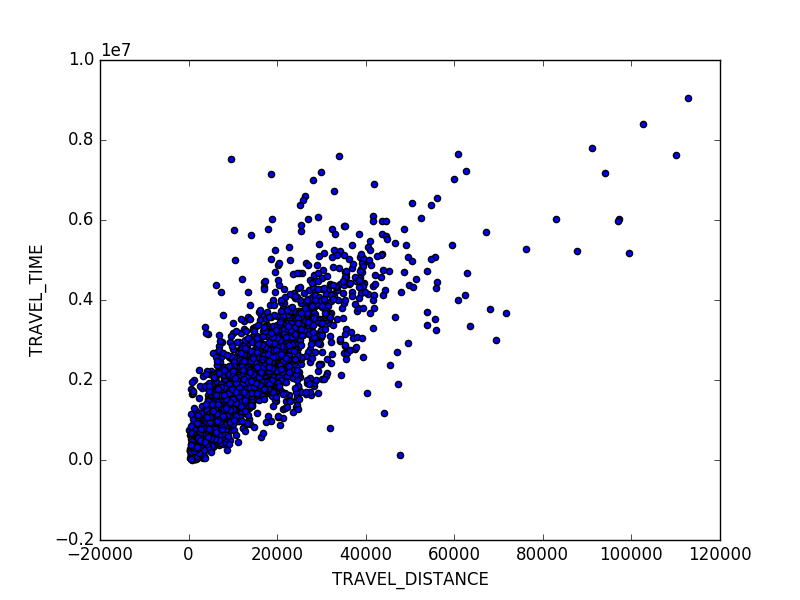
\includegraphics[width=.8\linewidth]{./images/distance_vs_time.png}
  \caption{Travel distance vs travel time. 2500 record sample.}
  \label{fig:preprocessing/distance_time_correlation}
\end{figure}

Travel time, travel distance, total transfer time and average transfer time where standardized by subtracting the mean of each distribution and forcing a unit standard deviation.

\begin{figure}[H]
  \centering
  \begin{subfigure}[b]{.45\textwidth}
  	\centering
  	\includegraphics[width=\linewidth]{"./images/Travel time_hist"}
  	\caption{Original}
  \end{subfigure}
  \begin{subfigure}[b]{.45\textwidth}
  	\centering
  	\includegraphics[width=\linewidth]{"./images/Travel time standardized_hist"}
  	\caption{Standarized}
  \end{subfigure}
  \caption{Time distribution before and after preprocessing. 2500 records sample.}
  	\label{fig:preprocessing/time}
\end{figure}

\begin{figure}[H]
  \centering
  \begin{subfigure}[b]{.45\textwidth}
  	\centering
  	\includegraphics[width=\linewidth]{"./images/Travel distance_hist"}
  	\caption{Original}
  \end{subfigure}
  \begin{subfigure}[b]{.45\textwidth}
  	\centering
  	\includegraphics[width=\linewidth]{"./images/Travel distance standardized_hist"}
  	\caption{Standarized}
  \end{subfigure}
  \caption{Distance distribution before and after preprocessing. 2500 records sample.}
  	\label{fig:preprocessing/distance}
\end{figure}

Figure \ref{fig:preprocessing/time} and \ref{fig:preprocessing/distance} show travel time and distance follow a truncated Gaussian distribution $\mathcal{N}(\mu = 1, \sigma^2 = 1)$. Since the nature of the data prevents negative values (time and distance must be positive), the original distribution is truncated at 0. Standardization maintains the shape of the distribution, but shifts and contracts it to be closer to zero values.

The mean travel time is ~55 minutes, and the mean travel distance is ~10 kilometers.  
 
\begin{figure}[H]
  \centering
  \begin{subfigure}[b]{.45\textwidth}
  	\centering
  	\includegraphics[width=\linewidth]{"./images/Total transfer time_hist"}
  	\caption{Original}
  \end{subfigure}
  \begin{subfigure}[b]{.45\textwidth}
  	\centering
  	\includegraphics[width=\linewidth]{"./images/Total transfer time standardized_hist"}
  	\caption{Standarized}
  \end{subfigure}
  \caption{Total transfer time distribution before and after preprocessing. 2500 records sample.}
  	\label{fig:preprocessing/transfer_time}
\end{figure}

\begin{figure}[H]
  \centering
  \begin{subfigure}[b]{.45\textwidth}
  	\centering
  	\includegraphics[width=\linewidth]{"./images/Average transfer time_hist"}
  	\caption{Original}
  \end{subfigure}
  \begin{subfigure}[b]{.45\textwidth}
  	\centering
  	\includegraphics[width=\linewidth]{"./images/Average transfer time standardized_hist"}
  	\caption{Standarized}
  \end{subfigure}
  \caption{Average transfer time distribution before and after preprocessing. 2500 records sample.}
  	\label{fig:preprocessing/transfer_avg}
\end{figure}

Figure \ref{fig:preprocessing/transfer_time} and \ref{fig:preprocessing/transfer_avg} show that transfer times, both total and average, follow distributions with very long tails. As mentioned before, most trips are performed without transfers, which explains that most of the trips have transfer times equal to zero. \selfnote{do not include transfer 0. focus on tail behavior}


\subsection{Attributes}
The spatial features to be included in the representation are:

\begin{enumerate}
\item Small traffic area
\item Middle traffic area
\item Big traffic area
\item Ring road
\item District
\item Mode
\item Line/Route
\item Stop
\end{enumerate}

These are repeated for boarding and alighting information.

The general trip features to be included in the representation are: 

\begin{enumerate}
\item Travel time
\item Travel distance
\item Transfer number
\item Transfer total time
\item Transfer average time
\item Start hour
\item End hour
\item Number of trips
\end{enumerate}

The attributes are of two types: numerical and categorical. Usually categorical should be done by one hot encoding. In this case it is not scalable.

\subsection{User cubes}

\begin{figure}[H]
  \centering
  \includegraphics[width=.9\linewidth]{"./images/Commuter Day"}
  \caption{Sample Day slice for random Commuter.}
  \label{fig:preprocessing/commuter}
\end{figure}

\begin{figure}[H]
  \centering
  \includegraphics[width=.9\linewidth]{"./images/Non-commuter Day"}
  \caption{Sample Day slice for random Non-commuter.}
  \label{fig:preprocessing/commuter}
\end{figure}


\newpage
\section{Commuters identification}
\label{sec:partII}

\subsection{Attributes correlation}

\begin{figure}[H]
  \centering
  \includegraphics[width=.9\linewidth]{"./images/General correlation"}
  \caption{Attributes correlation to each other and to label.}
  \label{fig:classification/correlation}
\end{figure}

\textbf{General}

\textbf{Temporal}

\textbf{Spatial}: Hierarchy in geographical areas causes correlation

\subsection{Feature selection}
Statistical correlation to label, f value of anova. chi 2 discarded because it focuses on times only
machine learning through trees
domain knowledge

Aggregation system. Each method's scores are normalized to add up to 1. Each contribute with equal weight. 

\begin{figure}[H]
  \centering
  \includegraphics[width=.9\linewidth]{"./images/scores"}
  \caption{Attributes scores.}
  \label{fig:classification/scores}
\end{figure}

Choose middle area and mode. 

\begin{figure}[H]
  \centering
  \includegraphics[width=.9\linewidth]{"./images/Selected features"}
  \caption{Visualization of samples and their labels after feature selection.}
  \label{fig:classification/tsne}
\end{figure}

\subsection{Model}
Take slices of cubes and flatten. 

We compare a single SVM, ensembled random forests. 

As suggested by Tu \cite{tu2016impact} results, the data is almost linearly separable thus simple classifiers such as decision trees may suffice. 



\subsection{Experiments}

\textbf{SVM}

Accuracy: 94.66\%

\begin{figure}[H]
  \centering
  \includegraphics[width=.9\linewidth]{"./images/SVM_Heatmap"}
  \caption{SVM confusion matrix.}
  \label{fig:classification/svm_confusion}
\end{figure}
  
\textbf{Random Forest}  

Accuracy: 97.54\%

\begin{figure}[H]
  \centering
  \includegraphics[width=.9\linewidth]{"./images/Random forest_Heatmap"}
  \caption{Random forest confusion matrix.}
  \label{fig:classification/rf_confusion}
\end{figure}


\textbf{AdaBoost}  

Accuracy: 98.24\%


\begin{figure}[H]
  \centering
  \includegraphics[width=.9\linewidth]{"./images/AdaBoost of decision trees_Heatmap"}
  \caption{Random forest confusion matrix.}
  \label{fig:classification/adb_confusion}
\end{figure}


\subsection{Discussion}
Random Forests deal well with categorical information. Adaboost deals well with missing information.

Overfitting



\newpage
\section{Commuters clustering}
\label{sec:partIII}

\subsection{Feature extraction}
The features to be fed into the clustering algorithms are obtained by dimensionality reduction. As mentioned before, convolutional filters can exploit local information.

\subsubsection{Convolutional filters}
In order to examine weekly patterns, our the first layer of convolutional filters will have an x dimension of 7 with a stride of 7. Assuming that only the hour previous and after a trip affects the trip, the filter will have a y dimension of 3 with a stride of 1. We do not perform padding, since this would have significant implications in the travel behavior of the user. 

Following this formula:

\begin{align*}
	output = \frac{input - filter}{stride} +1
\end{align*}

We find that the output size after the first convolution is $4 \times 22$. Considering 15 features, this reduces the dimensionality to $4 \times 22 \times 15 = 1320$

Goal is to have a $ 4 \times 3 \times 3 = 36$ structure

\technicalDoubt{what about depth? can I have a filter that is 8 units deep, with 8 stride (features are divided as 8 spatial boarding, 8 spatial alighting and 8 transfer related)? How could this be applied?}

\subsubsection{Autoencoder}
A neural network is constructed to apply the convolutional filter. After the convolution layer, ReLU is applied as activation function. 

TSNE results 

\subsection{Clustering}
Tuning

Evaluation

\subsection{Cluster analysis}

\subsection{Discussion}


\newpage
\section{Conclusion and future work}

Faulty data. Missing data from 9 to 16. Gap in between.

Zero values such as end hour, zero transfers and others. Same effect as "empty" bin. 

Overlapping trips. So far one trip per bin/hour. Possible solutions are to concatenate.

Standardization by day.

Selection over trip -> label. 

\newpage
\bibliography{mybib}{}
\bibliographystyle{plain}

\end{document}
